\chapter{MapReduce for mtDNA High Throughput Sequencing: mtDNA-Server}
\label{chap:NGS}

The first decoding of the full genome by the Human Genome Project was finished after 13 years (earlier as expected) in 2003 \cite{InternationalHumanGenomeSequencingConsortium2004}. Since then, not only the sequencing methods but also the algorithms for data processing improved constantly. Further the prices dropped from US\$3 billion to the long awaited \$1000 for sequencing a whole human genome (3.2 billion base pairs)\footnote{http://blogs.nature.com/naturejobs/2015/10/08/big-data-the-impact-of-the-human-genome-project/} generated within just hours/days. Therefore the bottleneck shifted from data generation to data processing. This is the result of the so called second generation or next-generation sequencing devices, which deploy a massively parallelization sequencing. Thereby millions of short reads are read out, and the data processing wouldn't be possible without the improved Bioinformatics and computer science based tools. 

To process this \textit{"data-flood"}, soon parallel computing architectures are required. Even though only about 1 percent of the complete genome is derived from the mitochondria, the higher content compared to the nuclear genome results in an increased file size. 

This Chapter presents a system called mtDNA-Server \cite{Weissensteiner2016b}. It was designed as Software as a Service, to process next-generation sequencing reads of mitochondrial DNA, independently of the sequencing strategy. Target mtDNA sequencing, whole genome sequencing (WGS) or whole exome sequencing (WES) data can be analyzed. Since mitochondria play an important role in cancer \cite{Brandon2006,He2010,Guo2012,KlossBrandstatter2010}, with this new high-coverage data, also deeper understanding in the development or progression of cancer can be provided. The debate whether mutations help drive the tumor, or are bystander events can now be explored with this new sequencing method \cite{McMahon2014,Kloss-Brandstatter2015}. Further scientific relevant questions are the influence of the mitochondrial genome in the process of aging or in other disease such as neurodegenerative diseases. Here, mtDNA-Server can help the researchers by hiding the complexity of the data processing and providing additional quality control, to avoid the publication of false positive results. 

\section{Background: Parallelism is the Key}
When Google described it's framework MapReduce in 2004 \cite{Dean2008}, the NGS devices began their triumphal procession of massively parallel sequencing (MPS). While the NGS devices produced parallel data of genomic sequences, the parallelism in the MapReduce programming paradigm is achieved by splitting data to key/value pairs which are processed in the Map phase and the Reduce function on huge clusters of commodity hardware. In 2009, first approaches based on MapReduce entered the field of genetics \cite{Schatz2009}. The term Cloud-computing got established shortly thereafter 2010 \cite{Schatz2010}. The same time our group began investigating the potential of MapReduce for Genomics with first results presented in 2011 \cite{DBLP:conf/gvd/SchonherrFWKSK11}. The presented solution in this chapter is based on Apache Hadoop and the execution framework Cloudgene \cite{Schonherr2012} developed by Sebastian Sch\"onherr and Lukas Forer as partial fulfillment of their PhD requirements. Cloudgene allows the straight-forward realization of MapReduced based workflows, based on a YAML\footnote{{http://www.yaml.org/}}-configuration files, thereby automatically generating the graphical user-interface. 

\section{Burrows-Wheeler vs. Hashing}
The alignment and mapping of short reads generated by NGS devices to a reference genome is crucial for identifying variants on the DNA or RNA. Therefore after the quality control of the raw files with tools such as FastQC\footnote{\url{(http://www.bioinformatics.babraham.ac.uk/projects/fastqc/)}}, sequence mapping is required. Various approaches for this task were designed, resulting in dozens of short read mapping tools  \cite{Hatem2013,Pabinger2013}, with different strength and weaknesses. The two most important classes are Hashing (of overlapping k-mer words) and Burrows-Wheeler Transformations. While Hashing is consuming more memory for large reference genomes, it is very fast for exact matches, and therefore best used for highly similar sequences (see Chapter \ref{chapterAlignment}). The reference size is however not an exclusion criteria for the mitochondrial genome with its small size of less than 17kb. This approach is applied in tools like SMALT, SOAP or SSAHA2. Burrows-Wheeler based approaches like BWA \cite{Li2009}, Bowtie \cite{Langmead2009} or SOAP2 are fast and show a high sensitivity, also for repetitive regions, where Hashing shows less sensitivity. The principal concept of Burrows-Wheeler Transformation is to compress an Suffix-Tree. Thereby the index itself can be compressed, by permuting the order of characters representing the nucleobases in such manner, that characters are resorted and ordered according repeats. For the herein presented solution, BWA MEM \cite{Li2013a} was considered to have the best trade-off between speed and accuracy and is largely accepted in the genetics field (e.g. used in the 1000 Genomes Project \cite{Abecasis2012}).

\section{Related Work}
Several tools for sequence alignment/mapping were developed with the increase of data generated by NGS devices. While most of the tools are written in C/C++, Python or Java very few tools came with a user-interface. Also most of those tools are developed for linear DNA, not considering the circular structure of mtDNA. While the alignment/mapping is just the first step for data processing, several other steps are required, to cover the spectrum from alignment to the representation and annotation of the variants. Those steps comprise the following classifications, whereby an extensive overview of the different tools per step can be found in Pabinger et al. \cite{Pabinger2013}. 
\begin{enumerate}\label{enum:NGS}
\item alignment/mapping of the raw reads to the reference genome considering the circular structure
\item sort the generated BAM file and process the mapped reads
\item perform a variant calling considering low level heteroplasmy, by applying specific models
\item classification of variants to haplogroups
\item perform a quality control in order to prevent misinterpretation of contamination 
\item annotate the variants and generate reports
\end{enumerate}

For scientists in the lab, where Linux-environments are often lacking, single tools or the complete pipelines are often not accessible. One initiative to make the creation of workflows/pipelines accessible to scientists in life science, is the \textbf{Galaxy Project} \cite{Goecks2010,Afgan2016}. Galaxy allows the generation of workflows in a graphical way, by providing a large selection of Bioinformatic applications, that can be connected interactively with "point and click". Galaxy got extended by Galaxy CloudMan \cite{Afgan2010}, which allows deploying computing cluster on the Amazon EC2 cloud infrastructure. The Galaxy group also published two workflows presented in \cite{Goto2011} and \cite{Dickins2014} where mitochondrial genomes from NGS devices was processed and the data as well as the pipeline was made freely available. The pipeline comprises 43 steps, that cover all the previously mentioned steps in NGS mtDNA analysis. For mapping BWA is used, the resulting SAM file gets filtered and converted to BAM file, the pileup file gets generated and several filter for forward and reverse reads are applied. A cleaned variant file with heteroplasmic levels that differ above 1\% from the reference base are reported as result.

\textbf{Mitoseek} \cite{Guo2013} was developed for exome and whole genome sequencing data of the mitochondrial genome. Mitoseek is written in Perl and combines several steps. As a first step, the already mapped BAM file gets extract mitochondrial reads that don't map to the nuclear DNA, due to the presence of Numts (nuclear copies of mitochondrial DNA) \cite{Parr2006, Dayama2014}. Basic quality control is performed by generating plots of the per base sequence quality as well as the length distribution of the reads.  Mitoseek also performs the variant calling and allows to detect 0.1 \% of heteroplasmy if the coverage of 10,000x is present. Besides the filters provided by the user, Mitoseek implements statistical frameworks for the assessment of heteroplasmy and also detects somatic mutations, by comparing tumor-benign pairs of samples. It however lacks a graphical user interface and does not allow to check for haplogroups.

One of the first tools with a convenient web-based user-interface for the analysis of mtDNA NGS data was presented in Zidhkov et al. \cite{Zhidkov2011}. \textbf{MitobamAnnotator} starts with the mapped BAM file to the rCRS or the Yoruba Sequence used in HG18 by using Samtools \cite{Li2009} to process the reads. It takes the user input for filtering by three different categories (high quality read parameters, consensus calling parameters and heteroplasmy parameters) and annotates the heteroplasmic variants with the scores and writes files for haplogroup classification in HaploGrep. It is however limited to one file per upload of 500MB. 

\textbf{MtoolBox} is a pipeline for heteroplasmy annotation and prioritization analysis of human mitochondrial variants in high-throughput sequencing \cite{Calabrese2014}. The workflow starts with BAM or FASTQ files and maps the raw reads with GSNAP \cite{Wu2010}. Besides the dependency to GSNAP, MToolBox which is written in Python relies on Samtools and MUSCLE \cite{Edgar2004}. It performs a realignment around known insertions and deletions based on the Genome Analysis Toolkit GATK \cite{McKenna2010} and marks duplicates based on the Picard Tools\footnote{\url{http://broadinstitute.github.io/picard}}. The variants are called by a fragment-classification tool to detect the heteroplasmic fraction (called HF) and the related confidence interval for each position of the mitochondrial genome. As a result a VCF file and the haplogroup assignment as well as the functional annotation (similar to  the information provided in MitImpact \cite{Castellana2014}) are generated. MToolBox is made available with a user-interface on MseqDR\footnote{\url{https://mseqdr.org/mtoolbox.php}} presented in Shen et al. \cite{Shen2015} .  

\textbf{mit-o-matic} defines itself as a comprehensive computational and experimental pipeline for clinical evaluation of mitochondrial variations from next-generation sequencing datasets \cite{Vellarikkal2015}. The pipeline comes with an online user-interface\footnote{\url{http://genome.igib.res.in/mitomatic}}. limited to file uploads of 25MB per sample of FASTQ files. Three mapping tools are directly supported to map the raw reads to the rCRS reference sequence: BWA, BOWTIE and MAQ. Option 2 accepts the parsed pileup file which is generated with the download version of mit-o-matic (available only after applying for a lincense), not limited to the 500x coverage otherwise. The variant calling is a done by calculating the percentages of reads showing the variant allele out of the total. Annotation is based on Mitomap\footnote{\url{http://www.mitomap.org}} presented in Lott et al.\cite{Lott2013} as well as mtDB\footnote{\url{http://www.mtdb.igp.uu.se/}}, MitoLSDB \cite{K2013} and Sift for predicting the functional effect of a heteroplasmic induced amino acid substitution. Haplogroup prediction is based on Mitotool \cite{Fan2011,Fan2013}. 

\textbf{LoFreq} \cite{Wilm2012} is not limited to mitochondrial genomes and is one of many variant caller available. It was however validated with mitochondrial genomes and was designed to detect 0.05\% of variants. It accepts the mapped BAM file and comes without the need of specifying any parameters. The variant calling is superior to the most herein presented related work. It is based on a Bernoulli trial, where success corresponds to the reference base, and failure to the variant base (K). A Poisson-binomial distribution handles each Bernoulli trial with distinct success probabilities and calculates the exact P-values for observing a variant base in a recursive way. Since this approach is $O(N^2)$ run time optimization were applied so that LoFreqs worst-case runtime is $O(KN)$. LoFreq's result is a VCF file, however without the required FORMAT and SAMPLE columns, since LoFreq was not designed for calling genotypes, but rather low-level variants.

Table \ref{comparisonRelatedWork} gives a summary of the herein outlined tools. Comparison to our mtDNA-Server cloud-application is made, with the method described in more detail in this Chapter.

\begin{table}[h]
\centering
\caption{Comparison of related work - the numbers in brackets represent the enumeration of the different steps in \ref{enum:NGS}}
\label{comparisonRelatedWork}
\begin{tabular}{|l|l|l|l|l|l|l|l|}
\hline
Feature & \begin{tabular}[c]{@{}l@{}}Gal\\ axy\end{tabular} & \begin{tabular}[c]{@{}l@{}}Mito\\ Seek\end{tabular} & \begin{tabular}[c]{@{}l@{}}M.Bam\\ Annot.\end{tabular} & \begin{tabular}[c]{@{}l@{}}MTool\\ Box\end{tabular}. & \begin{tabular}[c]{@{}l@{}}mit-o\\ matic\end{tabular} & LoFreq & \begin{tabular}[c]{@{}l@{}}mtDNA\\ Server\end{tabular}\\
\hline
FASTQ (1,2) & + & - & - & + & + & -& + \\
BAM (3) & + & + & + & + & - & +& + \\
Low-level (4) & + & + & + & + & - & +& + \\
Cont.Check(5) & + & - & - & - & - & -& + \\
Reports (6) & + & + & + & + & + & -& + \\
GUI & + & - & + & + & + & -& + \\
Haplogroups & - & - & + & + & + & -& + \\
Parallel & - & - & - & - & - & -& + \\
VCF & + & - & - & + & - & +& - \\
\hline
\end{tabular}
\end{table}
\section{mtDNA-Server: bringing MapReduce to NGS based mtDNA data}
Both areas of research, i.e. MapReduce for computer science and NGS for life sciences are well established. Our approach brings MapReduce to the field of genetics, and represents one of the first real use-case. By taking advantage of the Apache implementation Hadoop \cite{White2009}, our group previously implemented Cloudgene \cite{Schonherr2012}, a middle-layer to automatically generate the user interface. It was previously designed with two modules: Cloudgene-Cluster and Cloudgene-MapRed. While Cloudgene-Cluster was used to instantiate a cluster on a public cloud, like Amazon's EC2, Cloudgene-MapRed represents the layer between Hadoop and the mtDNA-Server application. It comes with its own workflow engine (a Directed Acyclic Graph Manager) and its own workflow definition language and enables to execute different applications on top of it in an independent manner. The Cloudgene API provides the means for the execution and monitoring of MapReduce jobs. It also handles the communication with the Hadoop cluster and provides a web interface for all job-related tasks  \cite{Weissensteiner2016b} (see section \ref{webservice}).
%rewritten from paper

mtDNA-Server represents such an application: it is an mtDNA analysis workflow starting with the raw data in FASTQ or BAM format and performs a variant calling that results in reliable detection of heteroplasmic sites and variants, contamination estimates and numerous QC statistics based on R \cite{R} and the knitr package\footnote{\url{http://yihui.name/knitr/}}. To take advantage of parallelism, mtDNA-Server supports the upload of several samples at once. Thereby each input file is further split into independent chunks (called intra-sample chunking) \cite{Weissensteiner2016b}. For parallelization, as earlier mentioned, the Hadoop MapReduce framework\footnote{\url{http://hadoop.apache.org/}} is used. Within Hadoop, a cluster of nodes, each consisting of several cores, processes the chunks (each chunk consisting of a 64 MB package of sequence reads) in parallel in the map function, which gets an input record and maps it to one or more key/value pairs. Thereafter the data is grouped and collected by the framework in the shuffle step and further analyzed or directly returned to the application in the reduce function, getting a single key and a list of values on which an operation can be performed (in this case: count the different nucleobases per position). The presented application is written in Java and a YAML file defines the workflow. The architecture of mtDNA-Server can be drafted in Figure \ref{fig:mtdna-server-architecture}. All MapReduce steps are highlighted with the bold lines i.e. (1) Read Alignment, Quality Control and (2) Heteroplasmy Detection. The contamination check is calculated on the Namenode, as well as the annotation of heteroplasmic sites. Both steps take advantage of the previously described HaploGrep in Chapter \ref{chap:NGS}, which was made available as console version for integrating it in pipelines. 
\begin{figure}[h]
    \centering
    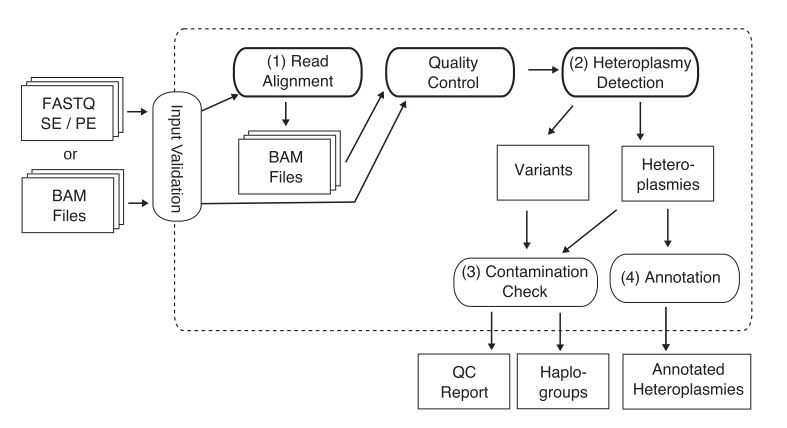
\includegraphics[width=1\textwidth]{images/mtdna-server.JPG}
    \caption[mtDNA-Server workflow for FASTQ and BAM input files]{mtDNA-Server workflow for FASTQ and BAM input files. Figure as represented in \cite{Weissensteiner2016b}}
    \label{fig:mtdna-server-architecture}
\end{figure}
\subsection{Input validation}
mtDNA-Server allows the upload of FASTQ files, the mapped SAM files or the binary mapped BAM files. The FASTQ files can be paired end or single end, SAM and BAM files are handled with the same input reader. As of May 2017, in total over 45,000 samples were processed - thereby 72\% of all samples were in SAM/BAM format, 12\% in FASTQ single end and 16\% of all uploaded samples were FASTQ paired end files. Depending on the user selected file format, the specific set of workflow steps is executed in parallel. The validation step verifies the selected file format and checks it by automatic format detection of the uploaded files. As a next validation step for the mapped SAM/BAM files, the header needs to contain the mitochondrial reference sequence with length according the rCRS or RSRS, being 16,569. Since the human reference genome until the Genome Reference Consortium Human genome build 37 (GRCh37 or hg19) used an African reference sequence for the mitochondrial genome (Yoruba reference \texttt{NC\_001807.4} with length 16,571. This reference is also accepted, and gets automatically converted to meet the nomenclature of the rCRS (\texttt{NC\_012920.1}). This is crucial for the post-processing steps, especially the generation of the HaploGrep files and the annotation of the amino acid changes. Listing \ref{listBAMheader} represents part of the SAM/BAM header and the required size for chrM = the mitochondrial genome (sometimes referred to as chromosome 26).

\begin{lstlisting}[caption=Header of SAM/BAM file expecting length (LN) 16569 or 16571 for chrM, label=listBAMheader]
@HD VN:1.5 SO:coordinate
@SQ    SN:chr1    LN:249250621
@SQ    SN:chr2    LN:243199373
...
@SQ    SN:chrM    LN:16569
\end{lstlisting}

\subsection{Parallel read alignment}
When the Input validation step completes successfully, the input data is put in the Hadoop Distributed File System (HDFS). If the input corresponds to FASTQ files, the raw sequences are mapped to the rCRS reference sequence automatically. This is done with BWA-MEM v 0.7.5 \cite{Li2013a} through the Java bindings (JNI) for bwa version of JBWA\footnote{\url{https://github.com/lindenb/jbwa}} by adapting it to run in the Hadoop environment. FASTQ files can be generated depending on the NGS devices in two different ways: either as paired-end reads (shown in simplified form: a DNA sequence gets read from both sides) or as single-end reads (DNA sequence is read from one side only). Paired-end reads are generally handled in two different files, and the ID of the reads in each file point to the corresponding forward and reverse reads.
The correct read pairs are identified by setting the Hadoop output key to the read name, as previously described \cite{Weissensteiner2016b, Pireddu2011}. Figure \ref{fig:mapreduce} gives an overview of the invoked map and reduce functions. This extra step is not required for single-end reads, were each chunk can be directly mapped with BWA-MEM, and the resulting SAM records are stored in the HDFS. The splitting of the chunks needed adoptions, since the FASTQ file consists of four lines in the file describing one read. After the generation of the SAM file, the BAM files are written, by using the secondary sort mechanism of Hadoop MapReduce. Thereafter, all steps are identical to the direct import of BAM files by the user, described in the next subsection.
\begin{figure}[!ht]
    \centering
    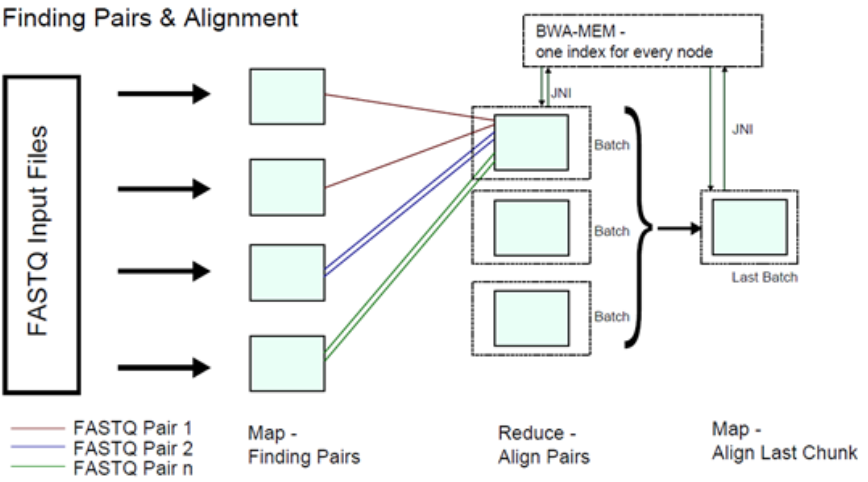
\includegraphics[width=1\textwidth]{images/mapreduce.png}
    \caption[Paired End Read Alignment with MapReduce]{Paired End Read Alignment with MapReduce - The Hadoop map function creates keys consisting of the read ID to sort read pairs. The reducer amounts the read pairs to a batch and executes it via a JNI method (JBWA) with BWA-MEM. Remaining reads are aligned within the Last-Batch method.  }
    \label{fig:mapreduce}
\end{figure}
\subsection{Quality Control}
During this QC step, the BAM input file gets analyzed and basic statistics are generated. This way, the user can get real-time feedback and gets a first idea on how good the data quality of the sequencing run was. These statistics include metrics on how many reads are mapped, how many duplicate reads were filtered or if a reference based issue was found. The example QC report for two samples from the 1000 Genomes project (IDs: HG00096 and HG00740) looks as presented in Figure \ref{fig:mtdna-server-qc}. The high amount of filtered reads indicates a low data quality (below Phred-Score Q20). If a run quits unexpectedly, the FWD Bases and REV Bases would show a significant difference in the amount.  
\begin{figure}[!ht]
    \centering
    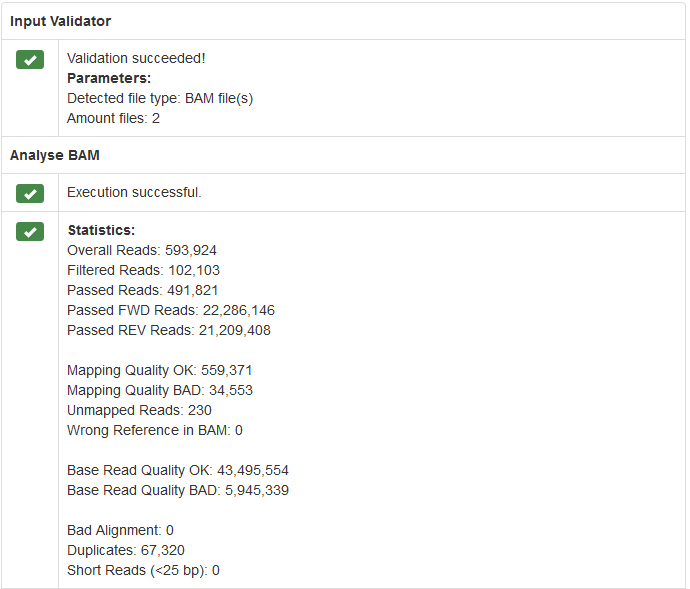
\includegraphics[width=1\textwidth]{images/mtdna-server-qc.png}
    \caption[Example statistics for 2 samples from 1000G]{Example statistics for 2 samples HG00096 and HG00740 from the 1000G data set}
    \label{fig:mtdna-server-qc}
\end{figure}
\subsection{Parallel processing of BAM file}\label{settings}
When the QC step finishes successfully, the BAM file is processed with Hadoop-Bam \cite{Niemenmaa2012}, which splits the BAM files across the nodes, as previously drafted. Each chunk is processed autonomously and filtered on read (=sequence of n-bases) and base (=the nucleotide A,C,G or T) level. mtDNA-Server filters reads with a mapping quality Phred score Q$<$20  and requires the minimum read length$<$25, as presented in \cite{Zhidkov2011}. Reads being marked as duplicates are also filtered within this step. mtDNA-Server does not search for duplicates on its own, only emits the marked as duplicates reads. Further, mtDNA-Server excludes all reads with an alignment Phred score Q$\leq$30 and applies the per-Base Alignment Quality (BAQ \cite{Li2011}) to all reads by default. BAQ reduces the false variant calls around indels (insertions and deletions) by performing a profile Hidden Markov Model. For this purpose, the GATK \cite{McKenna2010} BAQ implementation has been adapted in order to consider the circular structure of the mitochondrial genome. For each passed read, all bases with a quality Phred score Q $<$20 are also filtered. The remaining passed bases are counted per strand and per site, where the nucleobases are A, C, G, T, N (unknown base) or d (deletion). Each node provides a list of the sums over each bases (\textit{values}) per site (\textit{key}) per chunk.
When the reduce function processes the key/value pairs, in a first step the heteroplasmy rate is calculated and in a second step the homoplasmic (full allele substitution against the reference sequence).
\subsection{Variant calling}
For the calling of variants, we differentiate heteroplasmic variants from homoplasmic variants. For heteroplasmic variant calling, additional filters and methods are applied: in a first step, mitochondrial hotspots around the polymeric C tracts around site 310 as well as the N on 3107, causing issues with the alignment according to the rCRS are excluded. Sites with coverage $\leq$10 bases per strand are not considered for heteroplasmy detection. For all remaining sites the next filters are:

\begin{enumerate}
\item  a variant allele frequency (VAF) of $\geq$ 1\% for each strand independently  
\item  a variant allele count of three bases per strand 
\item  an Maximum-Likelihood (ML) model according \cite{Ye2014} is applied.The ML model takes sequencing errors per base into account and is applied to each strand \cite{Weissensteiner2016b}. The likelihood function is as follows:
\begin{equation}
  L(f)=\prod_{i=1}^{l} [(1-f) \epsilon_{i} + f(1-\epsilon_i)] \prod_{i=1}^{k} [(1-f) (1- \epsilon_{i}) + f(\epsilon_i)] 
\end{equation}
Where $l$ and $k$ represent the major and minor alleles respectively, $\epsilon$ the sequencing error probability and the parameter of interest is the major allele frequency $f$. 
All sites with a log likeli-hood ratio (LLR) was calculated as 
\begin{equation}
  LRR=\log L({\widehat{f}_{h_1}}) /  L({\widehat{f}_{h_0}}) 
\end{equation}
where $h_0$ represent the model for homoplasmy and $h_1$ the model for heteroplasmy. LLR $\geq5$ are tagged as heteroplasmic sites, which was defined as high-confidence heteroplasmy in \cite{Picardi2012}. 
\item  A strand bias score is applied to check the forward and reverse independently calculated. Since strands are analyzed independently, mtDNA-Server can filter all heteroplasmic sites with a strand bias score $<1$ \cite{Weissensteiner2016b,Guo2012}. The strand bias $SB$ is calculated as follows:
\begin{equation}\label{eq:llr}
  SB=\left| \frac{k_1}{l_1+k_1} - \frac{k_2}{l_2+k_2} \right| / \left(\frac{k_1 + k_2}{l_1+l_2+k_1+k_2}\right)
\end{equation}
where $k_1$ and $k_2$ represent the forward($_1$) and reverse($_2$) strand of the minor allele count, and $l_1$ and $l_2$ represent the forward($_1$) and reverse($_2$) strand of the major allele count. We ignored the presence of a third allele, which is likely the result of sequence or alignment errors.
\item Furthermore we calculate the binomial proportion confidence interval, depending on the coverage of the alleles: the Wilson Score Interval and the Agresti-Coull Interval as proposed in \cite{Calabrese2014}. 
Both are improvements of the normal approximation method of the binomial confidence interval:
\begin{equation}
\begin{split}
  BCI_{upper} = p + \left(z_{1- \frac{\alpha}{2}} \right)\sqrt[]{\frac{p (1-p)}{n} } \\ 
  BCI_{lower} = p - \left(z_{1- \frac{\alpha}{2}} \right)\sqrt[]{\frac{p (1-p)}{n} } 
\end{split}
\end{equation}
where $p$ is the heteroplasmy level of interest (minor alleles / all base counts), $n$ the base count of all bases on a specific site, and  $z_{1- \frac{\alpha}{2}}$ = $1.96$ for a $95\%$ confidence (which assumes an error level of 5\%) or 2.57 for 99\% confidence.
\item The heteroplasmy level (HET.LEVEL) is the calculated as the weighted mean of the minor variant alleles on the forward and reverse strand. 
\end{enumerate}
The files created for download are the unfiltered pileup format file, the annotated files for variants and the HaploGrep input files. Those are generated automatically and made available for sharing or direct download to the user.
\subsection{Contamination Check}
Mitochondrial genomes can be classified into haplogroups, as reported in Chapter \ref{chapterHaplogrep}. The concept that is applied here is that sample contamination can be seen based on a mixture of haplogroups manifesting as low-level heteroplasmy on the haplogroup defining variants, which is covered in more detail in the next Chapter \ref{chapterContamination}. 
\subsection{Annotation}\label{subs:annotation}
We tag positions in low complexity regions (LCR) \cite{Zhidkov2011} and known polymorphic nuclear mitochondrial insertions (NumtS) \cite{Dayama2014}. LCR tagging is particular necessary for Ion Torrent and Roche generated samples, showing an increased per-base error in homopolymeric stretches $geq$4 bases.  The annotation contains: the Map-Locus of the variant, the phylogenetic weight according Phylotree \cite{VanOven2009} as well as the Amino Acid Change, the MutPred-Score \cite{Li-mutpred2009} and the SelectionScore \cite{Pereira2011}.
\subsection{Web Service}
\label{webservice}
As previously mentioned, mtDNA-Server takes advantage of Cloudgene as the underlying platform to build a scalable web service including the automatically generated graphical user interface. mtDNA-Server has been integrated by using Cloudgene’s workflow definition language based in a YAML file and its plugin interface \cite{Schonherr2012, Weissensteiner2016b}. By integrating mtDNA-server as Cloudgene pipeline, it profits from features like user login, real-time feedback as well as data security. Moreover, it enables mtDNA-Server to assemble all possible heteroplasmic and homoplasmic sites, QC statistics, and various plots describing the data as well as contamination detection into an interactive graphical report that can be viewed directly in the web browser or can be shared with collaborators  \cite{Weissensteiner2016b}.
\section{Results}
\subsection{Data Import}
%The two major issues when we tried to publish mtDNA-Server in a first instance, were comments from the reviewers, concerning (i) file upload limitations and (ii) data sensitivity/privacy concerns. To address those issues, we added additional features to mtDNA-Server. 
mtDNA-Server accepts files from different input sources, with the typical file size as represented in Table \ref{mtDNAsource}: 
\begin{enumerate}[label=(\alph*)]
\item   local file upload via web: When using the file upload, data is imported from the users file system to the mtDNA-Server. One or several files can be selected and imported at once. The current upload limit is 5 GB. The limitation here is also the browser, allowing either 2GB upload (the case for Firefox but also more than 4GBs with Google Chrome). 
\item   local file upload via command line tool: mtDNA-Server supports users with high upload demands by providing a command line upload tool which can be downloaded from the mtDNA-Server website\footnote{\url{http://mtdna-server.uibk.ac.at/start.html}}. The upload tool automatically extracts all reads mapping to the mitochondrial genome, so that for some scenarios, only a small portion of the BAM file needs to be uploaded. The QC quality checks are performed locally and mtDNA-Server starts automatically when all checks are fulfilled. For this import, an index file (.BAI) is required for the BAM files. 
\item   import from SFTP Servers or HTTPS Web-Servers: A convenient way to upload data is by specifying a SSH server location. This can be achieved by selecting "Secure File Transfer Protocol" in the Run Screen of mtDNA-Server. The username and the password for the accessing Server are required. A URL consists of the server address followed by the full Unix path. Several paths can be specified in consecutive lines.
\item   import from FTP servers or HTTP Web-Servers: mtDNA-Server can directly work with public available data via HTTP or FTP. This is achieved by opening "URLS (HTTP)" in the dropdown menu and adding the file URLs in the text-area. The direct file-importer extracts only the mitochondrial part of a whole genome /exome BAM file specifies, in an automatic manner. 
\end{enumerate}

\begin{table}[h]
\centering
\caption{Data size and possible sources for mtDNA-Server for processing mitochondrial massive parallel sequencing data \cite{Weissensteiner2016b}}
\label{mtDNAsource}
\begin{tabular}{llll}
\hline
mtDNA data source &  Mean Coverage & BAM file size & run time\\
\hline
Ancient DNA & $\leq$ 100-fold&  $<$10 MB  & $<$ 1 min.\\
Whole exome sequencing &$\leq$ 1,000-fold&  $<$20 MB  & $<$ 1 min.\\
Whole genome low coverage & $\leq$ 3,000-fold & 1-80 MB  & 1 min.\\
Whole genome high coverage & $\leq$ 20,000-fold & approx. 200MB & 3 min. \\
Targeted mtDNA sequencing &$\sim$50,000-fold & up to 1 GB  & 7 min.
\end{tabular}
\end{table}
%Direct file uploads are especially convenient for small sample sizes ($<$100 MB)  \cite{Weissensteiner2016b}. For large samples sizes, mtDNA-Server provides the import tool as well as the web importer from sftp / https or ftp / http to upload large datasets, often already present on Servers. 
To address concerns regarding data privacy and sensitivity, we implemented a wide array of security measures: the HTTPS protocol is used for securing the complete communication with the server. The uploaded input data is deleted  by the system itself as soon as a job terminates. The resulting files are available on the server for a limited period of 7 days. Thereafter all data are erased automatically. The data can also be deleted immediately by the user after downloading or inspecting the results online. Results derived from the public mode are protected by encrypted token URLs only accessible by the user itself \cite{Weissensteiner2016b}.

\subsection{Results and Data Export}
The results generated by mtDNA-Server can be accessed in an interactive report summarizing all findings. Further all the underlying data are provided for download. The HTML report generated in $R$ with $RMarkdown$ based on the $knitr$ package includes all graphical elements directly in this file. The additional files provided for download represent the  heteroplasmic and homoplasmic variants detected by the earlier described settings in \ref{settings}, the HaploGrep input file as well as the related haplogroup classification result file based on Phylotree 16. Further the raw pileup file is made available for download, including base position counts per sample and per site by reporting the forward and reverse LLR as presented in equation \ref{eq:llr}. 
%A SMTP can be configured in the Admin panel of mtDNA-Server to notify the user by sending an email, once a job has finished successfully. 
The HTML report itself presents several quality control (QC) measures  \cite{Weissensteiner2016b}: 
\begin{enumerate}[label=\textbf{QC.\arabic*}]
\item An overview of the selected base-quality based on the ratio of mapped to filtered reads, see Figure \ref{fig:mtdna-server-qc}. 
\item A responsive table listing all heteroplasmic variants, which can be searched, filtered or sorted by the user directly in the browser. 
\item A frequency table listing heteroplasmic sites found in more than two samples, which could indicate potential artefacts. 
\item \label{item:boxplot} A boxplot of the minor allele frequences summarizing the heteroplasmy levels per sample, not considering the reference base.
\item \label{item:barplot}A bar plot of the heteroplasmic sites found per sample: samples showing a large number of heteroplasmic could indicate issues while mapping/artefacts or sample mix ups that need to be checked.  
\item \label{item:maplocus}The map-loci of heteroplasmic sites: here the heteroplasmic sites are represented according the occurrence on the different loci over the whole mitochondrial genome with its coding- and non-coding regions.
\item An interactive table of resulting haplogroups with the HaploGrep quality score (see Chapter \ref{chapterHaplogrep}), the coverage information for each sample, based on the mean forward and reverse coverage over the whole genome, as well as the coverage of the least covered position and the coverage over the whole genome in absolute numbers, which can help especially for ancient mtDNA or mtDNA data derived from exome sequencing, where the mtDNA often is not covered on every site. 
\item  A contamination table indicating potential sample mix-ups, detected on phylogenetic issues, based on 5,437 haplogroups present in Phylotree. 
\item  Coverage-plots for each sample, that highlights issues in targeted re-sequencing studies. Incorrect concentrations of the PCR products results as shifts in the coverage of the used fragments (see Figure \ref{item:coverageplot}). 
\item  An interactive table for homoplasmic sites. For each variant the haplogroup defining status is represented in form of (yes, no and hotspot mutation (the latter does not have any impact on the haplogroup classification) and yield information regarding amino acid changes, phylogenetic weights as presented in HaploGrep 2 and pathogenicity scores and the pathogenicity scores as described in Section \ref{subs:annotation}. Figure \ref{fig:mtdna-server-plots} includes four plots from the final HTML report \cite{Weissensteiner2016b}.
\end{enumerate}
\begin{figure}[!ht]
    \centering
    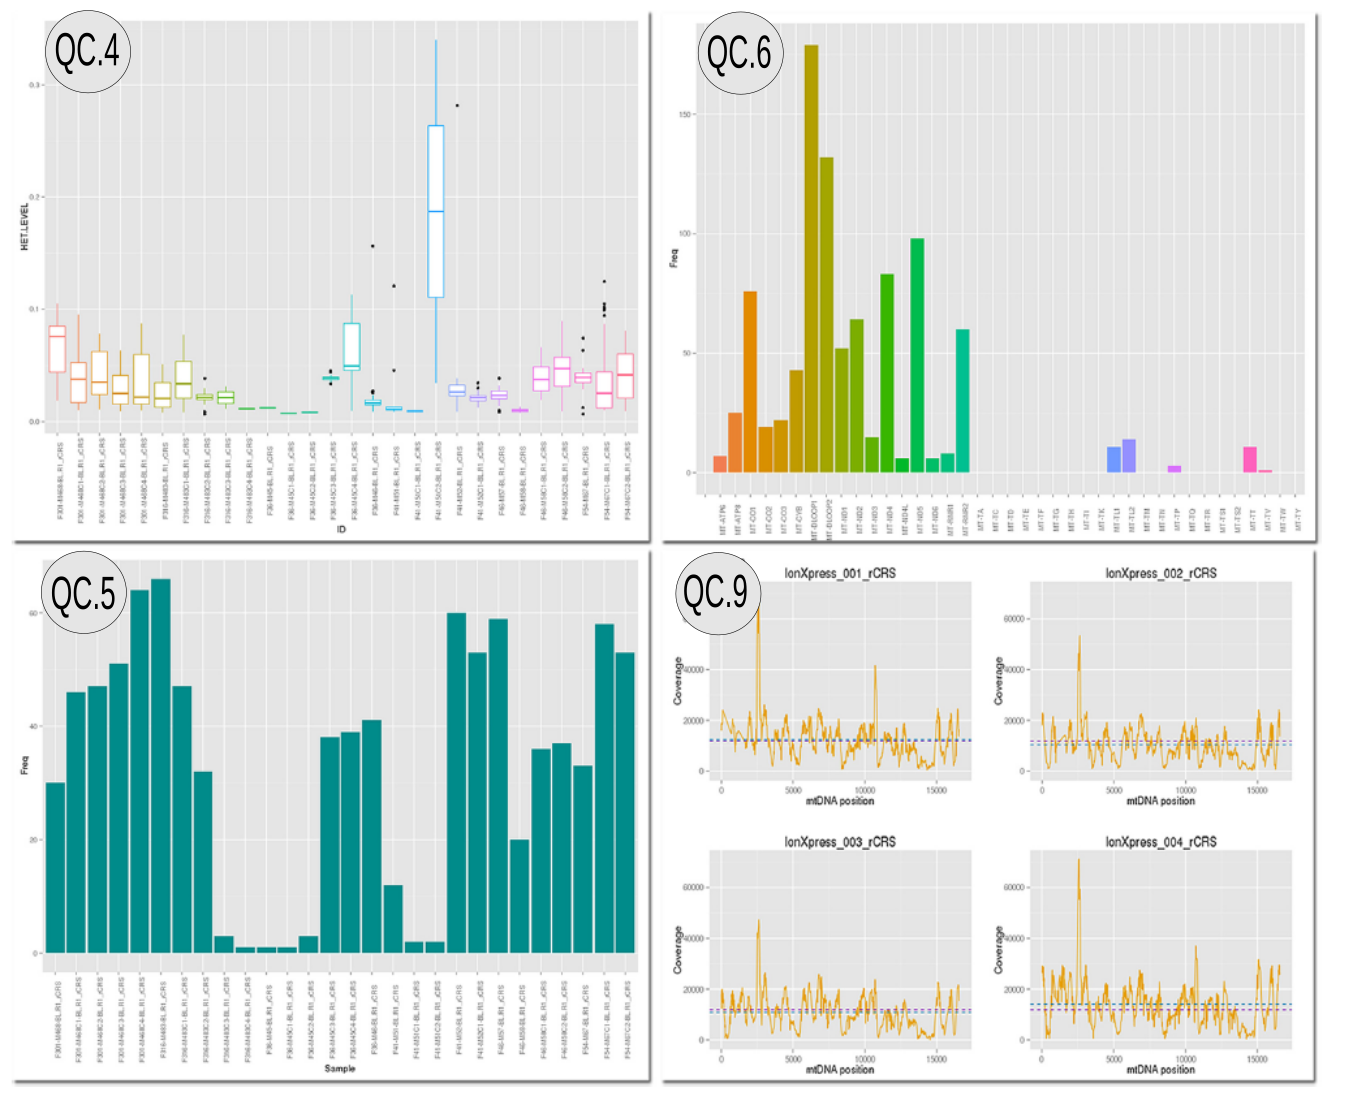
\includegraphics[width=1\textwidth]{images/mtdna-server-plots.png}
    \caption[Plots of the final HTML report]{Four plots of the final HTML report: Boxplot as described in \ref{item:boxplot}, frequency of the minor variant allele independent of reference as a bar plot \ref{item:barplot}, the map locus of the heteroplasmic variants (homoplasmy not considered) on the mitochondrial genome over all analyzed samples \ref{item:maplocus} and the coverage plots for per each sample, indicating the mean coverage over all samples and the mean coverage over all bases \label{item:coverageplot}.}
    \label{fig:mtdna-server-plots}
\end{figure}
\subsection{Validation}
In order to validate our herein presented heteroplasmy detection pipeline, we performed several validation steps and generated data in the lab, based on two blood samples. The concept was presented in our validation study \cite{Kloss-Brandstatter2015}, were we analyzed 28 samples of benign and cancer tissues from oral squamous cell carcinoma on both Sanger as well as Illumina HiSeq 2500 NGS devices. We also applied the mtDNA-Server pipeline within this publication for generating the results. To validate mtDNA-Server we generated 4 different sample-mix ups on the Illumina HiSeq 2500, and on the IonTorrent
PGM, which are also publishe in \cite{Weissensteiner2016b,Kloss-Brandstatter2015}. We run the same samples also on the SOLiD 5500xl, the Ion Torrent Proton, the Illumina MiSeq (with different chemistry) as well as one mix-up on the Oxford Nanopore MinION with the R7 chemistry. The results of the latter devices are part of a publication currently in progress and not reported within this work. The two samples got mixed in the laboratory as follows, by generating artificial contaminations: 
\begin{itemize}
\item Mix1 – 1:2 (50\%) 
\item Mix2 – 1:10 (10\%) 
\item Mix3 – 1:50 (2\%) 
\item Mix4 – 1:100 (1\%)
\end{itemize}
The two Samples were analzed in a prior study \cite{KlossBrandstatter2010}, and the sequences were deposited in GenBank with the following accession numbers:
\begin{enumerate}
\item Sample: HM625679.1\footnote{\url{http://www.ncbi.nlm.nih.gov/nuccore/301505851}} - Homo sapiens isolate Lab002 mitochondrion, complete genome  belonging to haplogroup U5a2e
\item Sample: KC286589.1\footnote{\url{http://www.ncbi.nlm.nih.gov/nuccore/445067603}} - Homo sapiens isolate Lab011 mitochondrion, complete genome  belonging to haplogroup H1c6
\end{enumerate}
We also had the runs of the un-mixed samples Lab002 and Lab011 and could detect low level of heteroplasmic variants that were excluded from the validation (i.e. in Sample Lab002 the heteroplasmic variants on position  15372 and in the Sample Lab011 the sites 7076, 9462, 11150, 15236 and 16129, found as private heteroplasmic mutations in the 1-3\% level). The 27 expected sites that differentiate the two profiles are on position 73, 151, 152, 477, 2706, 3010, 3197, 3768, 5979, 7028, 9145, 9477, 11467, 11719,
12308, 12372, 13617, 14766, 14793, 15289, 16189, 16234, 16256, 16270, 16311, 16362 and 16526 according the rCRS reference sequence, see Figure \ref{fig:mtdna-mix-ups}. 

\begin{figure}[!ht]
    \centering
    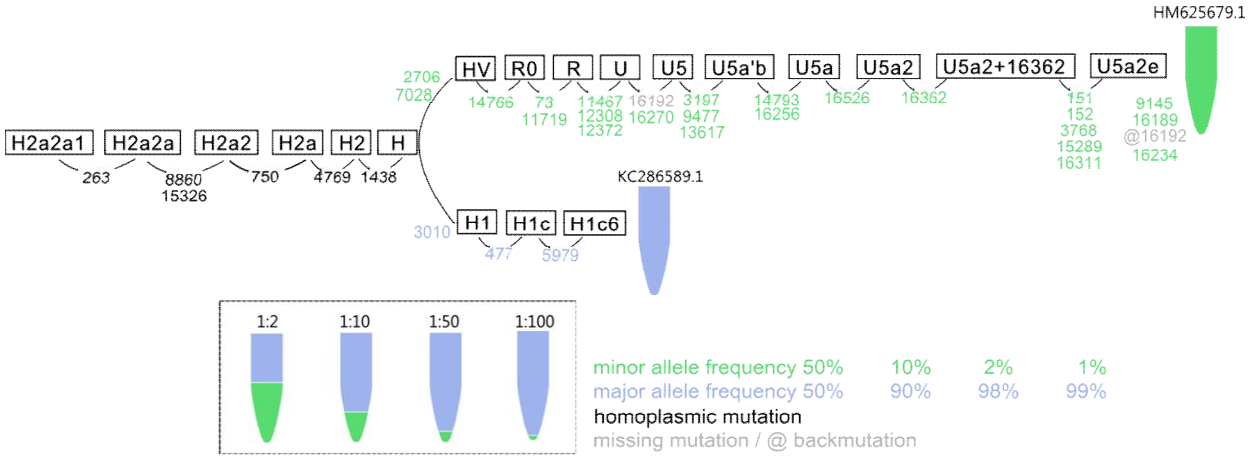
\includegraphics[width=1\textwidth]{images/mix-ups.png}
    \caption[Sample mixtures in the lab]{Two samples HM625679.1 and KC286589.1 as mixed in the lab. The profile of HM625679.1 (green) gets diluted down to 1\% level in the lab. The sites correspond the rCRS, and are either heteroplasmic (green or blue) according the mixture level or homoplasmic (=black, shared by both profiles, and expected as full base substitutions according the rCRS)} 
    \label{fig:mtdna-mix-ups}
\end{figure}
The Illumina HiSeq 2500 run yielded a mean coverage of 50,000x over the 6 samples (2 un-mixed and the 4 mix-ups) with a raw file size of the FASTQ files of 2GB per sample. The Ion Torrent PGM generated data on the Ion 318 Chip with a mean coverage of 5,000 fold over the same samples, with a BAM file size of 100MB per sample, already mapped with the Ion Torrent Suite. We converted the BAM files back to FASTQ files, for better comparison of the two devices, to exclude the impact of different mappers on the result. Both sets of files were run with the same parameters on mtDNA-Server and the results compiled based on comparing the expected to the detected heteroplasmic sites. For this purpose we determined the sensitivity (or recall) \textit{true positives rate}, the specificity (true negatives rate) and the precision (\textit{positive predictive value}). Listing \ref{eq:sensitivity} represents the definitions of the used performance metrics. 
\begin{equation}\label{eq:sensitivity}
\begin{split}
  Sensitivity =  \frac{number\ of\ true\ positives}{number\ of\ true\ positives\ + number\ of\ false\ negatives}\\ \\
  Specifity =  \frac{number\ of\ true\ negatives}{number\ of\ true\ negatives\ + number\ of\ false\ positives}\\  \\
  Precision = \frac{number\ of\ true\ positives}{number\ of\ true\ positives\ + number\ of\ false\ positives}
\end{split}
\end{equation}
The first validation was performed by comparing the Illumina HiSeq files after mapping with the same version of BWA MEM 0.7.5 to LoFreq, which is able of ultra-sensitive variant detection. Table \ref{table:illumina} shows the result based on the metrics presented for the Illumina HiSeq data. Table \ref{table:pgm} highlights the results for the Ion Torren PGM data.
\begin{table}[h]
\centering
\caption{Performance comparison between mtDNA-Server and LoFreq on the Illumina HiSeq 2500 mtDNA data}
\label{table:illumina}
\begin{tabular}{l|lll|lll}
\multicolumn{5}{c}{mtDNA-Server} &    {LoFreq} \\
\hline
\begin{tabular}[c]{@{}l@{}}Illumina\\ mix-up \end{tabular}  &  $Precis.$ & $Sensitiv.$ & $Specif.$  &  $Precis.$ &  $Sensitiv.$ & $Specif.$ \\
\hline
1:2 &   \textbf{100\%} &  \textbf{100\%}  & \textbf{100\%} &   93.1\%  & \textbf{100\%}   &   99.9\% \\
1:10 &  \textbf{100\%} &  \textbf{92.6\%}  & \textbf{100\%} &  89.3\%   &  \textbf{92.6\%}  &   99.9\% \\
1:50 &  \textbf{100\%} &  \textbf{92.6\%}  & \textbf{100\%}&   82.8\%  &  88.9\%  &   99.9\% \\
1:100 & \textbf{100\%} &  85.2\%  & \textbf{100\%} &  83.9\%   & \textbf{96.3\%}   &  99.9\%   
\end{tabular}
\end{table}
\begin{table}[h]
\centering
\caption{Performance comparison between mtDNA-Server and LoFreq on the Ion Torrent PGM mtDNA data}
\label{table:pgm}
\begin{tabular}{l|lll|lll}
\multicolumn{5}{c}{mtDNA-Server} &    {LoFreq} \\
\hline
\begin{tabular}[c]{@{}l@{}}PGM\\ mix-up \end{tabular}  &  $Precis.$ & $Sensitiv.$ & $Specif.$  &  $Precis.$ &  $Sensitiv.$ & $Specif.$ \\
\hline
1:2 &   \textbf{100\%} &  \textbf{88.89\%}  & \textbf{100\%} &  \textbf{100\%} & 81.48\%   &   \textbf{100\%} \\
1:10 &  \textbf{100\%} &  \textbf{81.48\%}  & \textbf{100\%} &  \textbf{100\%}  &  \textbf{81.48\%}   &   \textbf{100\%} \\
1:50 &  \textbf{100\%} &  \textbf{77.78\%}  & \textbf{100\%}&   \textbf{100\%} &  55.56\% &   \textbf{100\%} \\
1:100 & \textbf{100\%} &  \textbf{59.26\%}  & \textbf{100\%} &  \textbf{100\%}  & 11.11\% &  \textbf{100\%}   
\end{tabular}
\end{table}

As can be seen from the results, mtDNA-Server yields results that are more conservative: rather than finding all false negatives, it has the advantage of finding no false positives in this validation. The lack of not finding the true negatives relates to the BAQ which is applied as default in mtDNA-Server, which in this specific experiment shows some drawbacks. The diluted sample Lab002 shows 2 point mutation on site 151 and 152, as well as in the C-stretch around 16189 which are filtered too rigorously. On the other hand, LoFreq detects more false positives in the Illumina runs and even more false negatives in the PGM runs. In conclusion, both methods show a similar level of specificity and precision, but mtDNA-Server is slightly outperforming LoFreq regarding the sensitivity on both data sets from the NGS devices under investigation. This can come to additional costs if heteroplasmic variants are reassessed with a different method, for instance with Droplet Digital PCR or the Sequenom Platform, able to analyze specific sites, where the primers need to be known. 
\subsection{ Pipeline Performance Comparison }
For comparison with the presented tools in the related work section, two independent data sets were analyzed again with LoFreq and additionally with mit-o-matic, MToolBox, Galaxy Naive Variant Caller and  MitoSeek. The evaluation accessed the heteroplasmic sites found per tool. The evaluation shows that mtDNA-Server is the most accurate heteroplasmic variant calling pipeline over the analyzed data sets, with perfect precision, indicating the least false positive hits are found with the herein described method.

Since the mix-ups generated in the lab, that we used for validation were too large for upload on most of the different tools, we used two smaller publicly available data sets. The first was the high and low coverage data for sample HG00096 from the 1000 Genomes Project Phase 1, the second was a tumor/benign sample pair from the Cancer Genome Atlas \cite{Chang2013}, presented in \cite{Guo2013}.

The following parameters were used for the evaluation in order to reproduce the results:
\begin{enumerate}


\item MitoSeek (version 1.3)
\begin{lstlisting}
perl mitoSeek.pl -i <input.bam> -t 4 -sb 0 -hp 1 -d 5 -str 4 -sp 1 -sa 0
\end{lstlisting}
\item MToolBox on MSeqDR
\begin{lstlisting}
Input format: BAM 
reference sequence: hg19+rCRS 
Filtering and extra option: none 
Minimum distance of ins/dels from read end: 5 bps
Heteroplasmy threshold for FASTA consensus sequence: 0.8
\end{lstlisting}
\item Galaxy Naive Variant Caller
\begin{lstlisting}
Minimum base quality =20
Minimum mapping quality = 20
Minimum number of reads needed to consider a REF/ALT needed = 20 
ploidy = 1
\end{lstlisting}
\item Mit-o-matic\\
The files were converted to the required FASTQ format with BEDTools \cite{Quinlan2010} BamToFastq prior analysis.
\begin{lstlisting}
Read length: 101, 
Data: SingleEnd,
Alignment Tool: BWA
Heteroplasmy cut-off: 10% (default) as well as 1% 
\end{lstlisting}
For HG00096 which was too big for upload (exceeding the 25MB upload limit), we used the command-line version with the following parameters:
\begin{lstlisting}
perl mitomatic.pl -c -t bwa -o se -f 10 -d hg00096_10 -i HG00096.fastq
\end{lstlisting}
\item LoFreq
 \begin{lstlisting}
lofreq call HG00096.bam -o HG00096.vcf -f rCRSreference.fasta
\end{lstlisting}
\item  MitoBamAnnotator\\
Unfortunately we were not able to run either of the samples on MitobamAnnotator, ending up with a timeout of the server.
\item \textbf{mtDNA-Server}:
For mtDNA-Server no further parameters needed to be adjusted.
\end{enumerate}

\begin{table}[h]
\centering
\caption[Expected and detected heteroplasmic variants in sample HG00096]{Expected and detected heteroplasmic variants in sample HG00096 for different tools. Mutations with bold number are expected. Transversions only found on one strand are considered as artefacts and marked with $\star$. Error hot spot mutations reported by Li et al. \cite{Li2010} are marked with $\star \star$. }
\label{table:hg00096}
\begin{tabular}{c|c|cccccc}
\hline
Mutation & Exp. & LoFreq & \begin{tabular}[c]{@{}l@{}}Gal\\ axy\end{tabular} & \begin{tabular}[c]{@{}l@{}}Mito\\ Seek\end{tabular} & \begin{tabular}[c]{@{}l@{}}MTool\\ Box\end{tabular} & \begin{tabular}[c]{@{}l@{}}Ye\\ et al\end{tabular} & \begin{tabular}[c]{@{}l@{}}mtDNA\\ -Server\end{tabular} \\
\hline
1456 T/C & \textbf{1.0\%} & & & & 1.2\% & & 1.0\%\\
2746 T/C & \textbf{1.8\%} & 2.3\% & 2.5\% &2.4\% & 2.4\% & 2.3\% & 2.5\%\\
3200 T/C &\textbf{0.9\%} & & & & 1.00\% & & 1.02\%\\
12410 A/G & \textbf{1.0\%} & 1.3\% &1.3\%  & 1.2\% & 1.0\% & & 1.1\%\\
14071 A/G &\textbf{1.0\%} & 1.0\% & 1.2\% & & 1.2\%& & 1.1\%\\
14569 G/A &\textbf{50.2\%} & 57.6\% & 57.7\% & 58.0\% & 59.3\% &56.2\%& 57.6\% \\
15463 A/G & \textbf{0.9\%} & & & & 1.3\% & 1.08\% &1.3\%\\
16093 T/C& \textbf{56.8\%} & 60.2\% & 60.9\% & & 60.2\% & 59.5\% &59.6\% \\
16360 C/T &\textbf{39.4\%} & 39.4\% & 38.8\%& &  39.5\% & 37.8\% &38.6\% \\
3488 T/A$\star$ & & & & 1.1\% & 1.1\% &  \\
6419 A/C$\star$  & &  & 4.5\% & 1.5\%& 1.7\% \\
10306 A/C $\star \star$& & & 6.3\% & 2.5\% & 1.8\% &  \\

\end{tabular}
\end{table}
For the validation purpose we analyzed the sample HG00096 high coverage ($\sim$ 15,000 x) as our gold standard with LoFreq (column Exp. in Table \ref{table:hg00096}) and compared the results with the low coverage data (mean coverage 1,300x) to LoFreq, Galaxy Naive Variant Caller, MitoSeek, MToolBox on MSEQDR, the result as presented in Ye et al. \cite{Ye2014} and mtDNA-Server.  Mit-o-matic resulted in over 528 heteroplasmic sites by applying a 1\% heteroplasmic threshold and  20 heteroplasmic sites with a 10\% threshold, with a wrong resulting haplogroup U8b1b1 instead of the expected H16a1 and was therefore excluded.\\

As a next validation, a pair of mtDNA sequences from an exome sequencing study of a benign/tumor Breast cancer sample from  the Cancer Genome Atlas \cite{Chang2013} was assessed (sample TCGA-BH-A0BM-01A-11W-A071-09 = brca\_tumor with a mean coverage of 200x and TCGA-BH-A0BM-10A-01W-A071-09 = brca\_benign with a mean coverage of 50x).
Figure \ref{fig:coverage_brca} shows the coverage plots directly generated in mtDNA-Server. With the two low coverage data presented, the variant calling is more error prone to artefacts and errors from the NGS devices and therefore presents a good comparison basis. 
\begin{figure}[!ht]
    \centering
    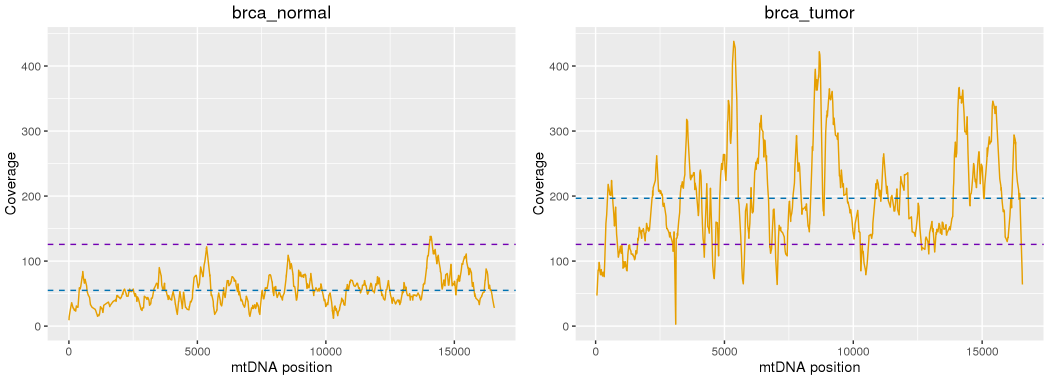
\includegraphics[width=1\textwidth]{images/coverage-brca.png}
    \caption[Coverage-plot generated by mtDNA-Server ]{Coverage-plot generated by mtDNA-Server of the two samples brca\_normal and brca\_tumor. The dotted line in purple shows the mean coverage over all analysed samples. The dotted line in turquoise shows the mean coverage for this specific sample.}
    \label{fig:coverage_brca}
\end{figure}
After analyzing the samples on mit-o-matic, Galaxy Naive Variant Caller (Galaxy NVC), LoFreq, MToolBox and mtDNA-Server the precision (Prec.) and sensitivity (Sens.) and specificity (Spec.) were estimated for both Samples. Table \ref{table:brca} represents the results of the metrics. In order to estimate the values, the results from LoFreq were used as the gold-standard, however ignoring the heteroplasmic variant on 10306 A/C which was shown to be an error hot spot by Li et al. \cite{Li2010}. 

\begin{table}[h]
\centering
\caption{Precision and Sensitivity based on the tumor-benign Breast-Cancer sample}
\label{table:brca}
\begin{tabular}{l|lll|lll}
\multicolumn{5}{c}{brca\_normal} &   {brca\_tumor}  \\
\hline
Pipeline &  $Prec.$ & $Sens.$ & $Spec.$  &  $Prec.$ & $Sens.$ & $Spec.$ \\
\hline
Galaxy NVC &    100\% &  100\% &  100\%  &   100\% &  62.5\% &  99.9\% \\
mit-o-matic &   0.17\% &  100\% &  99.9\%  &   71.4\% & 62.5\% & 99.9\% \\
MToolBox &      100\% &  100\% &  100\%  &   100\% & 100\% & 100\%\\
MitoSeek&       0\% &  0\% &  99.9\%  &   0\% & 0\% & 99.9\%\\
mtDNA-Server &  100\% &  100\% &  100\%  &   100\% &   100\% &   100\% \\
\end{tabular}
\end{table}
Detailed information on the variants found with each pipeline are provided in the Supplemental Material of the paper\footnote{\url{http://nar.oxfordjournals.org/content/suppl/2016/04/15/gkw247.DC1/SupplementaryMaterial.pdf}}. This evaluation again shows the poor performance of mit-o-matic, and surprisingly shows that a naive variant calling as performed with Galaxy is outperforming it. MToolBox and mtDNA-Server show similar results as LoFreq. MToolBox found additional 3 heteroplasmic variants that could be contributed to length heteroplasmy. But without further investigating the positions, they were not considered in this validation. 
\subsection{Scalability}
For the performance of the scalabilty mtDNA-Server was tested with an increasing amount of data size. Testing the scalability of the other pipelines is quite challenging, since often no batch processing is supported and samples can be only uploaded using a web interface. We performed two tests, one starts the whole steps with the Input of FASTQ files, the second test is with the BAM files from 1000 Genomes Project Phase 3. 

\subsubsection{Testing FASTQ paired-end (PE) samples}
High Coverage Illumina data (Illumina HiSeq 2500) from an in-house study \cite{Kloss-Brandstatter2015} with a mean coverage of $\sim$ 35,000 fold where used to validate the performance for the distributed alignment.
mtDNA-Server automatically detects paired-end data and adds an alignment step based on BWA-MEM 0.7.5. The Cluster Setup comprised a 3 Nodes Hadoop MapReduce Cluster with 30 CPUs in total and 2GB RAM per Node.
\begin{table}[h]
\centering
\caption{mtDNA-Server wall-time for FASTQ samples}
\label{table:fastq}
\begin{tabular}{lll}
Number of Samples  &  Datasize & Execution Time \\
\hline
10 &   6.2 GB &  30 min 10 sec \\
20 &  12 GB &  56 min 37 sec   \\
40 &  19 GB &  2 h 9 min 39 sec  \\
80 & 36 GB &  4 h 5 min 21 sec   
\end{tabular}
\end{table}

When taking a closer look at the run with the 80 FASTQ paired-end samples, mtDNA-Server provides the information for each step in the workflow, as presented in listing \ref{list80fastq}  

\begin{lstlisting}[caption=Execution times of workflow-steps in analysis of 80 FASTQ samples with mtDNA-Server, label=list80fastq]
Align                             [1 h 19 min 29 sec]
Sort BAM                          [1 h 48 min 2 sec]
Analyse BAM                       [54 min 6 sec]
Detect Heteroplasmy               [28 sec]
Haplogroup Detection              [8 sec]
Haplogroup Contamination Check    [20 sec]
Report Creation                   [54 sec]
Sending Mail                      [2 sec]
\end{lstlisting}

\subsubsection{Testing 1000G Phase1 BAM data}	
Data (up to 800 samples) were downloaded from the European Bioinformatics Institute FTP Server\footnote\url{ftp://ftp.1000genomes.ebi.ac.uk/} including Illumina and Roche data, in order to check for the scalability. Samtools was used for the download, by limiting to the mitochondrial genome reads only. As represented in Table \ref{table:bam} and in Figure \ref{fig:scalability} mtDNA-Server scales well with the amount of BAM samples. 
\begin{table}[h]
\centering
\caption{ mtDNA-Server wall-time for 1000 G Phase 1 BAM data}
\label{table:bam}
\begin{tabular}{lll}
Number of Samples  &  Datasize & Execution Time \\
\hline
50 &   1.8 GB &  3 min 26 sec\\
100 &  3.5 GB &  5 min 48 sec  \\
200 &  6.9 GB &  10 min 25 sec  \\
400 & 14 GB &  20 min 9 sec \\
800 & 27 GB & 38 min 54 sec
\end{tabular}
\end{table}

\begin{figure}[!ht]
    \centering
    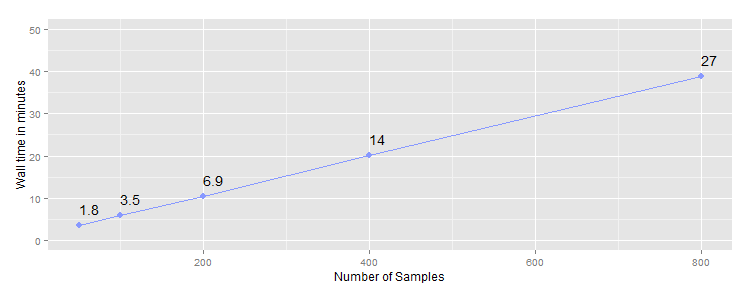
\includegraphics[width=1\textwidth]{images/scalability.png}
    \caption[Scalability of the mtDNA-Server pipeline]{Scalability of the Pipeline: Data from table \ref{table:bam} represented as x/y plot, where the points are denoted with the filesize in GB} 
    \label{fig:scalability}
\end{figure}
% DATA FOR PLOT IN R
% samples =c(50, 100, 200, 400, 800)
% size = c(1.8, 3.5, 6.9, 14, 27)
% df =data.frame(samples, size, timeMin)
% timeMin= c(3+(26/60), 5+(48/60), 10+(25/60), 20+(9/60), 38 + (54/60))
% ggplot(df, aes(x=samples, y=timeMin)) +  geom_line(aes(group=1), colour="#8899ff") +  geom_point(size=3, colour="#8899ff") +  xlab("Number of Samples") +  ylab("Wall time in minutes") + geom_text(aes(label=size),hjust=0, vjust=-1) +   ylim(0, 50) 

\section{Conclusion and Outlook}
In this chapter the "mtDNA-Server" (published in \cite{Weissensteiner2016b}) was described. It is a free and reproducible web service available on \url{http://mtdna-server.uibk.ac.at} for the complete mitochondrial NGS data analysis workflow, based on MapReduce. The focus is on the reliable detection of heteroplasmic variants as well as contamination in the samples. Complicated preprocessing steps are hidden to non-domain experts. The results highlight the accurate detection of variants (hetero- and homoplasmic) but also shows the scalability of the method with the increase amount of samples. mtDNA-Server has been developed in cooperation with the University of Michigan (Center for Statistical Genetics), the Medical University of Innsbruck and the University of Innsbruck, Institute of Computer Science with the Group of Database and Information Systems also providing the Hardware for this service.
Two important aspects need to be considered when providing such a free service:
\begin{enumerate}
\item Scalability of the service: All computational intensive steps are parallelized with Hadoop MapReduce and executed graphically with the Hadoop framework Cloudgene \cite{Schonherr2012, Weissensteiner2016b}. This framework is also used as the underlying framework for a heavily used service, the Michigan imputation Server \cite{Das2016} with over 10 million imputed genomes\footnote{\url{https://imputationserver.sph.umich.edu} accessed May 2017}.
\item Data Sensitivity: A wide array of security measures are in force \cite{Weissensteiner2016a}. Both data for input and output is removed from our servers as soon it is no longer needed. To upload and download data, users must register with a unique e-mail address and strong password or store the encrypted token URLs only accessible by the user who uploaded the data. Users can only download results for samples that they have uploaded; no other server users will be able to access their data.
\end{enumerate}

As of May 2017 over 45,000 samples got processed from scientists around the world and more than 400 users registered on the site. User registration is however not demanded to submit jobs. There's some more work to be addressed in the near future:

 Currently mtDNA-Server is focusing on the point mutations only. Insertions and deletions are not considered in the current version. This will be implemented in the near future (deletions are already emitted in the pileup file).
 
 Annotation of the heteroplasmic sites will be extended to phylogenetic scores and some pathogenicitiy scores, as already done in the homoplasmic variants. 

VCF file support, which should allow export of this file. While there is no current standard on how to write heteroplasmic variants, the VCF format presented in \cite{Calabrese2014} can be supported.

Since many researchers are not allowed to upload data to a remote destination we also plan on providing a Docker Image\footnote{\url{https://www.docker.com/}} for local usage. This allows to provide incremental updates to all users.  








